\begin{center}
 \textsc{Физбой, 11 класс. Финал.}
\end{center}
\vspace{0.01cm}
\hrule
\parindent=0mm

\taskpic{Определите сопротивление полубесконечной цепочки между точками
  $A$ и $B$, если сопротивление каждого звена равно $R$.}{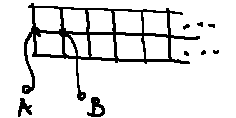
\includegraphics{fb11_1.pdf}}

\taskpic{Человек, стоя на краю высокого обрыва, смотрит на ровное
  плоское дно котлована шириной $L$, заполненного водой глубины
  $h$. Высота обрыва $H$. Размеры котлована удовлетворяют неравенствам
  $L \gg H \gg h$. Показатель преломления воды равен $n$. Как зависит
  от расстояния до обрыва видимая глубина котлована?}{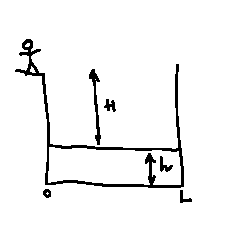
\includegraphics{fb11_2.pdf}}

\task{ По диаметру астероида, имеющего форму шара, проходит узкий
  тоннель. С поверхности астероида в тоннель бросили камень, сообщив
  ему скорость, равную первой космической для этого астероида. Через
  какое время камень вернётся назад? Известно, что минимальный период
  обращения космических объектов вокруг астероида равен
  $T_0$. Астероид состоит из однородного вещества, а влияние
  гравитационного поля других небесных тел мало. \\
  \textit{Примечание.} Площадь эллипса $S=\pi ab$, где $a,b$ --- длины
  полуосей эллипса.  }

\task{
  На расстоянии $H$ от бесконечной проводящей плоскости находится
  точечный заряд $q_0$. Найти, на каком расстоянии от проекции заряда
  на плоскость в эту плоскость войдёт силовая линия, вышедшая из
  заряда параллельно плоскости. 
}

\task{
  Один конец тонкой гибкой верёвки с линейной плотностью $\rho$ тянут
  с постоянной горизонтальной скоростью на высоте $H$ над шероховатой
  поверхностью. Второй конец верёвки свободен. Длина части верёвки,
  соприкасающейся с поверхностью, равна $l_1$. Найдите длину верёвки
  $l_2$, не касающейся поверхности. Коэффициент трения скольжения
  верёвки по поверхности равен $k$. 
}

\task{
  Предположим, что создан материал с необычной зависимостью
  коэффициента теплопроводности $k$ от температуры. Пластину из такого
  материала поместили между двумя стенками вплотную к ним. Температуры
  стенок поддерживаются постоянными: $T_1 = 160 K$ и $T_2 = 500 K$
  соответственно. Какой тепловой поток установится между стенками,
  если толщина пластины $d=1 \mbox{ см}$, а её площадь $S= 100 \mbox{
    см}^2$? Найдите температуру в среднем продольном сечении пластины
  ($x=d/2$). \\
\textit{Указание.} Тепловой поток $P$ сквозь тонкий слой вещества,
площадь которого равна $S$, а толщина $dx$, равный количеству теплоты,
проходящему через этот слой в единицу времени, прямо пропорционален
разности значений температуры его поверхностей $dT$ и обратно
пропорционален его толщине: $P = - k S \dfrac{dT}{dx}$, где $k$ ---
коэффициент теплопроводности вещества. 
}

\begin{center}
  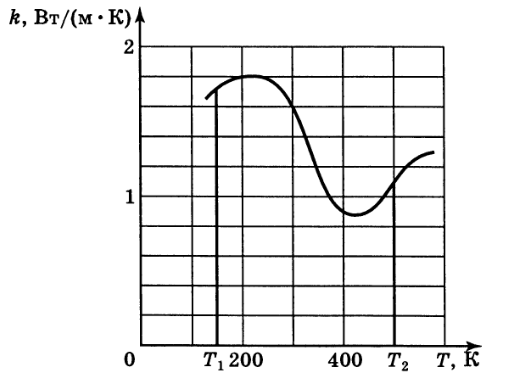
\includegraphics[width=6cm]{fb11_6.png}
\end{center}\setcounter{notask}{1}
